\documentclass[12pt]{article}

% TEMPLATE DEFAULT PACKAGES
\usepackage{amssymb,amsmath,amsfonts,eurosym,geometry,ulem,graphicx,color,setspace,sectsty,comment,natbib,pdflscape,array,adjustbox}

% ADDED PACKAGES FOR THIS MANUSCRIPT
\usepackage{palatino,newtxmath,multirow,titlesec,threeparttable,tabu,booktabs,titlesec,threeparttable,mathtools,bm,bbm,subcaption,pdflscape,tcolorbox,mathrsfs,tikz,graphicx}
% endfloat,

\usepackage{afterpage}
\usepackage[hyphens]{url}
\usepackage[margin=1cm]{caption}

\usepackage[draft]{hyperref}
\newcommand{\tim}{$\,\times\,$}
% FIGURES & TABLES CAPTION STYLING
\captionsetup[figure]{labelfont={bf},name={Figure},labelsep=period}
\captionsetup[table]{labelfont={bf},name={Table},labelsep=period}

% SECTION TITLE SETTINGS
\titlelabel{\thetitle.\enskip}
\titleformat*{\section}{\large\bfseries}
\titleformat*{\subsection}{\normalsize\bfseries}

% COLUMN TYPES
\newcolumntype{L}[1]{>{\raggedright\let\newline\\\arraybackslash\hspace{0pt}}m{#1}}
\newcolumntype{C}{>{\centering\arraybackslash}p{5.2em}}
\newcolumntype{D}{>{\centering\arraybackslash}p{5em}}
\newcolumntype{R}[1]{>{\raggedleft\let\newline\\\arraybackslash\hspace{0pt}}m{#1}}


% MARGINS AND SPACING
\normalem
\geometry{left=1.1in,right=1.1in,top=1.0in,bottom=1.0in}
\setlength{\parskip}{2.5pt}

% SPECIAL CELL 
\newcommand{\specialcell}[2][c]{%
	\begin{tabular}[#1]{@{}l@{}}#2\end{tabular}}

% NO INDENT ON FOOTNOTES
\usepackage[hang,flushmargin]{footmisc}

\begin{document}


\begin{figure}
\centering
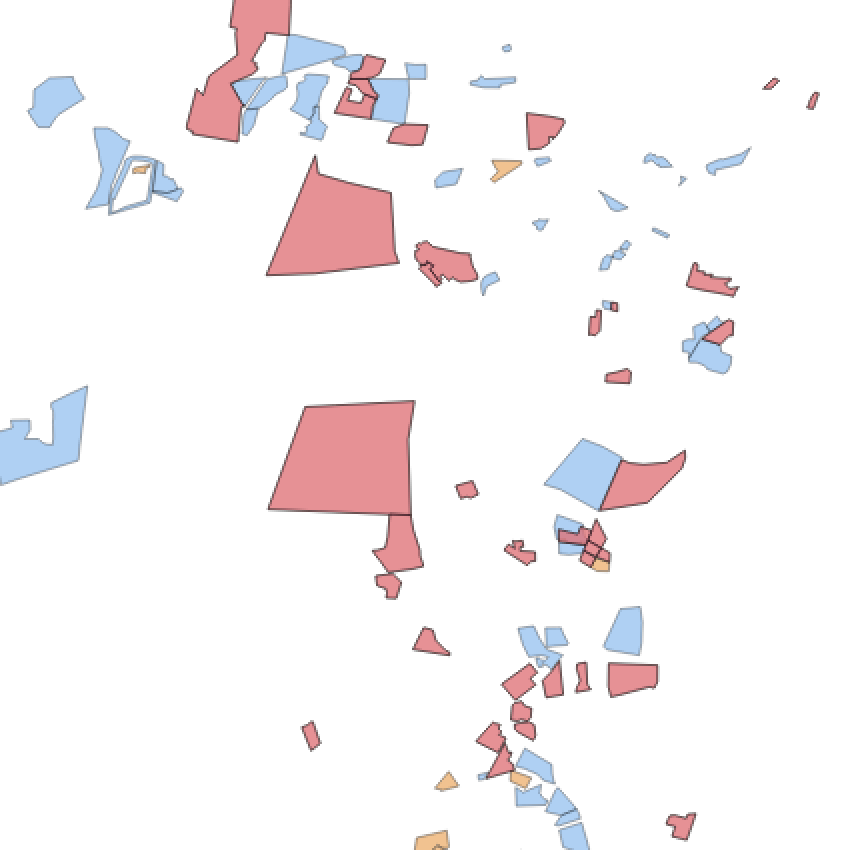
\includegraphics[scale=.4]{screenshot.png}
\begin{itemize}
\item Blue: constructed
\item Pink: unconstructed
\end{itemize}
\end{figure}

\begin{itemize}
	\item Current distance to boundary method is weird
		\begin{enumerate}
			\item intuitively : lots of projects clustered around each-other, close distances are way overweighted, while the further distances are representing weird spots (like bottom left corner)?
			\item economically : people don't care about ``which point is exactly closest to me'' but instead care about what share of my neighborhood is composed of project houses
			\item datawise : the plots don't look great; constructed are so much higher than unconstructed at baseline, and change gradients look weird past 1000-1200 meters (figures on next page)
				\begin{itemize}
					\item (one idea: estimate in first differences controlling for baseline housing density to account for the fact that places with high density at baseline might just naturally grow slower)
				\end{itemize}
		\end{enumerate} 
	\item 

\end{itemize}

\pagebreak

\begin{figure*}
        \centering
        \caption[ Pre-Period Housing Densities in Constructed and Unconstructed Projects Areas ]
        {\small Pre-Period Housing Densities in Constructed and Unconstructed projects } 
        %\vspace{2mm}
        \begin{subfigure}[b]{0.495\textwidth}
            \centering
            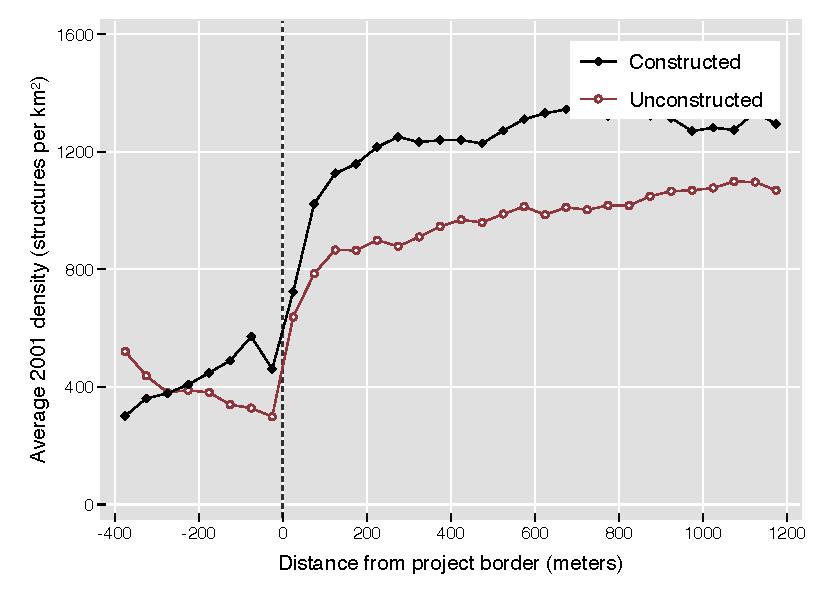
\includegraphics[width=\textwidth,trim={0.3cm .3cm 0.1cm 0cm}, clip=true]{figures/bblu_for_pre_means_4.pdf}
            \caption[Network2]%
            {{\small pre-period formal housing density}}    
            \label{fig:prefor}
        \end{subfigure}
        \hfill
        \begin{subfigure}[b]{0.495\textwidth}  
            \centering 
            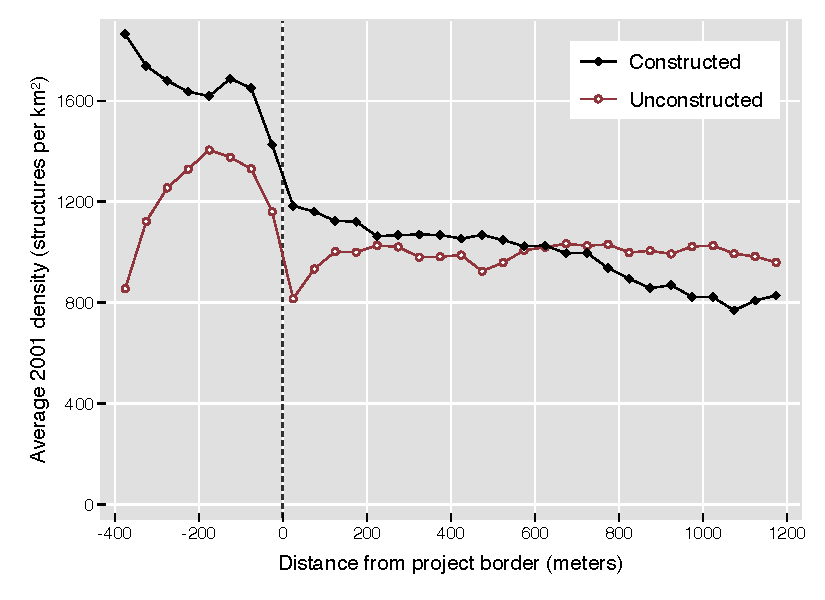
\includegraphics[width=\textwidth,trim={0.3cm .3cm 0.1cm 0cm}, clip=true]{figures/bblu_inf_pre_means_4.pdf}
            \caption[]%
            {{\small pre-period informal housing density}}    
            \label{fig:preinf}
        \end{subfigure}
        \label{fig:rawbblumeans}
        \vspace{-6mm}
    \end{figure*} 


\begin{figure*}
        \centering
        \caption[ Changes in Housing Densities in Constructed and Unconstructed Projects Areas]
        {\small Housing Densities in Constructed and Unconstructed projects } 
        %\vspace{2mm}
        \begin{subfigure}[b]{0.495\textwidth}   
            \centering 
            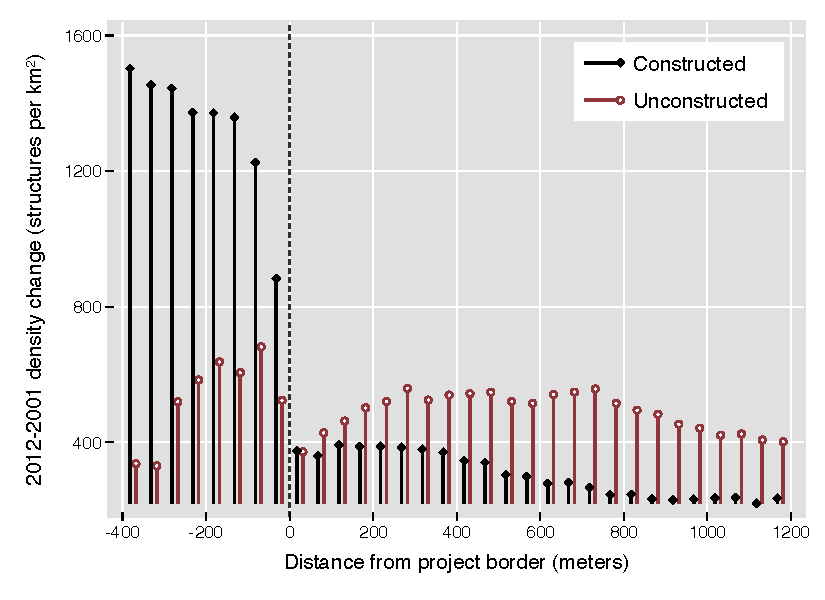
\includegraphics[width=\textwidth,trim={0.3cm .3cm 0.1cm 0cm}, clip=true]{figures/bblu_for_rawchanges_4.pdf}
            \caption[]%
            {{\small formal housing density change}}    
            \label{fig:forchange}
        \end{subfigure}
        \hfill
        \begin{subfigure}[b]{0.495\textwidth}   
            \centering 
            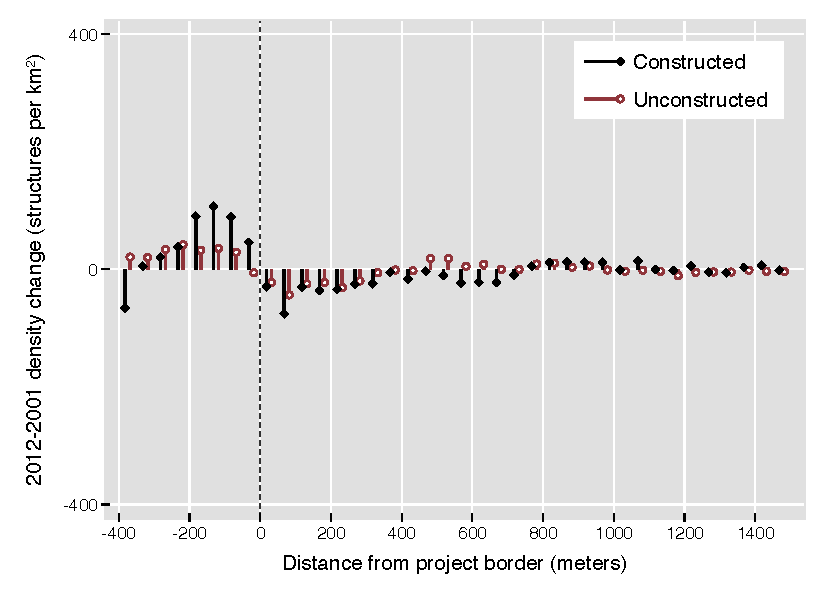
\includegraphics[width=\textwidth,trim={0.3cm .3cm 0.1cm 0cm}, clip=true]{figures/bblu_inf_rawchanges_4.pdf}
            \caption[]%
            {{\small informal housing density change}}    
            \label{fig:infchange}
        \end{subfigure}
        \label{fig:rawbblumeanschange}
        \vspace{-6mm}
    \end{figure*} 


\pagebreak



\begin{figure}
\centering
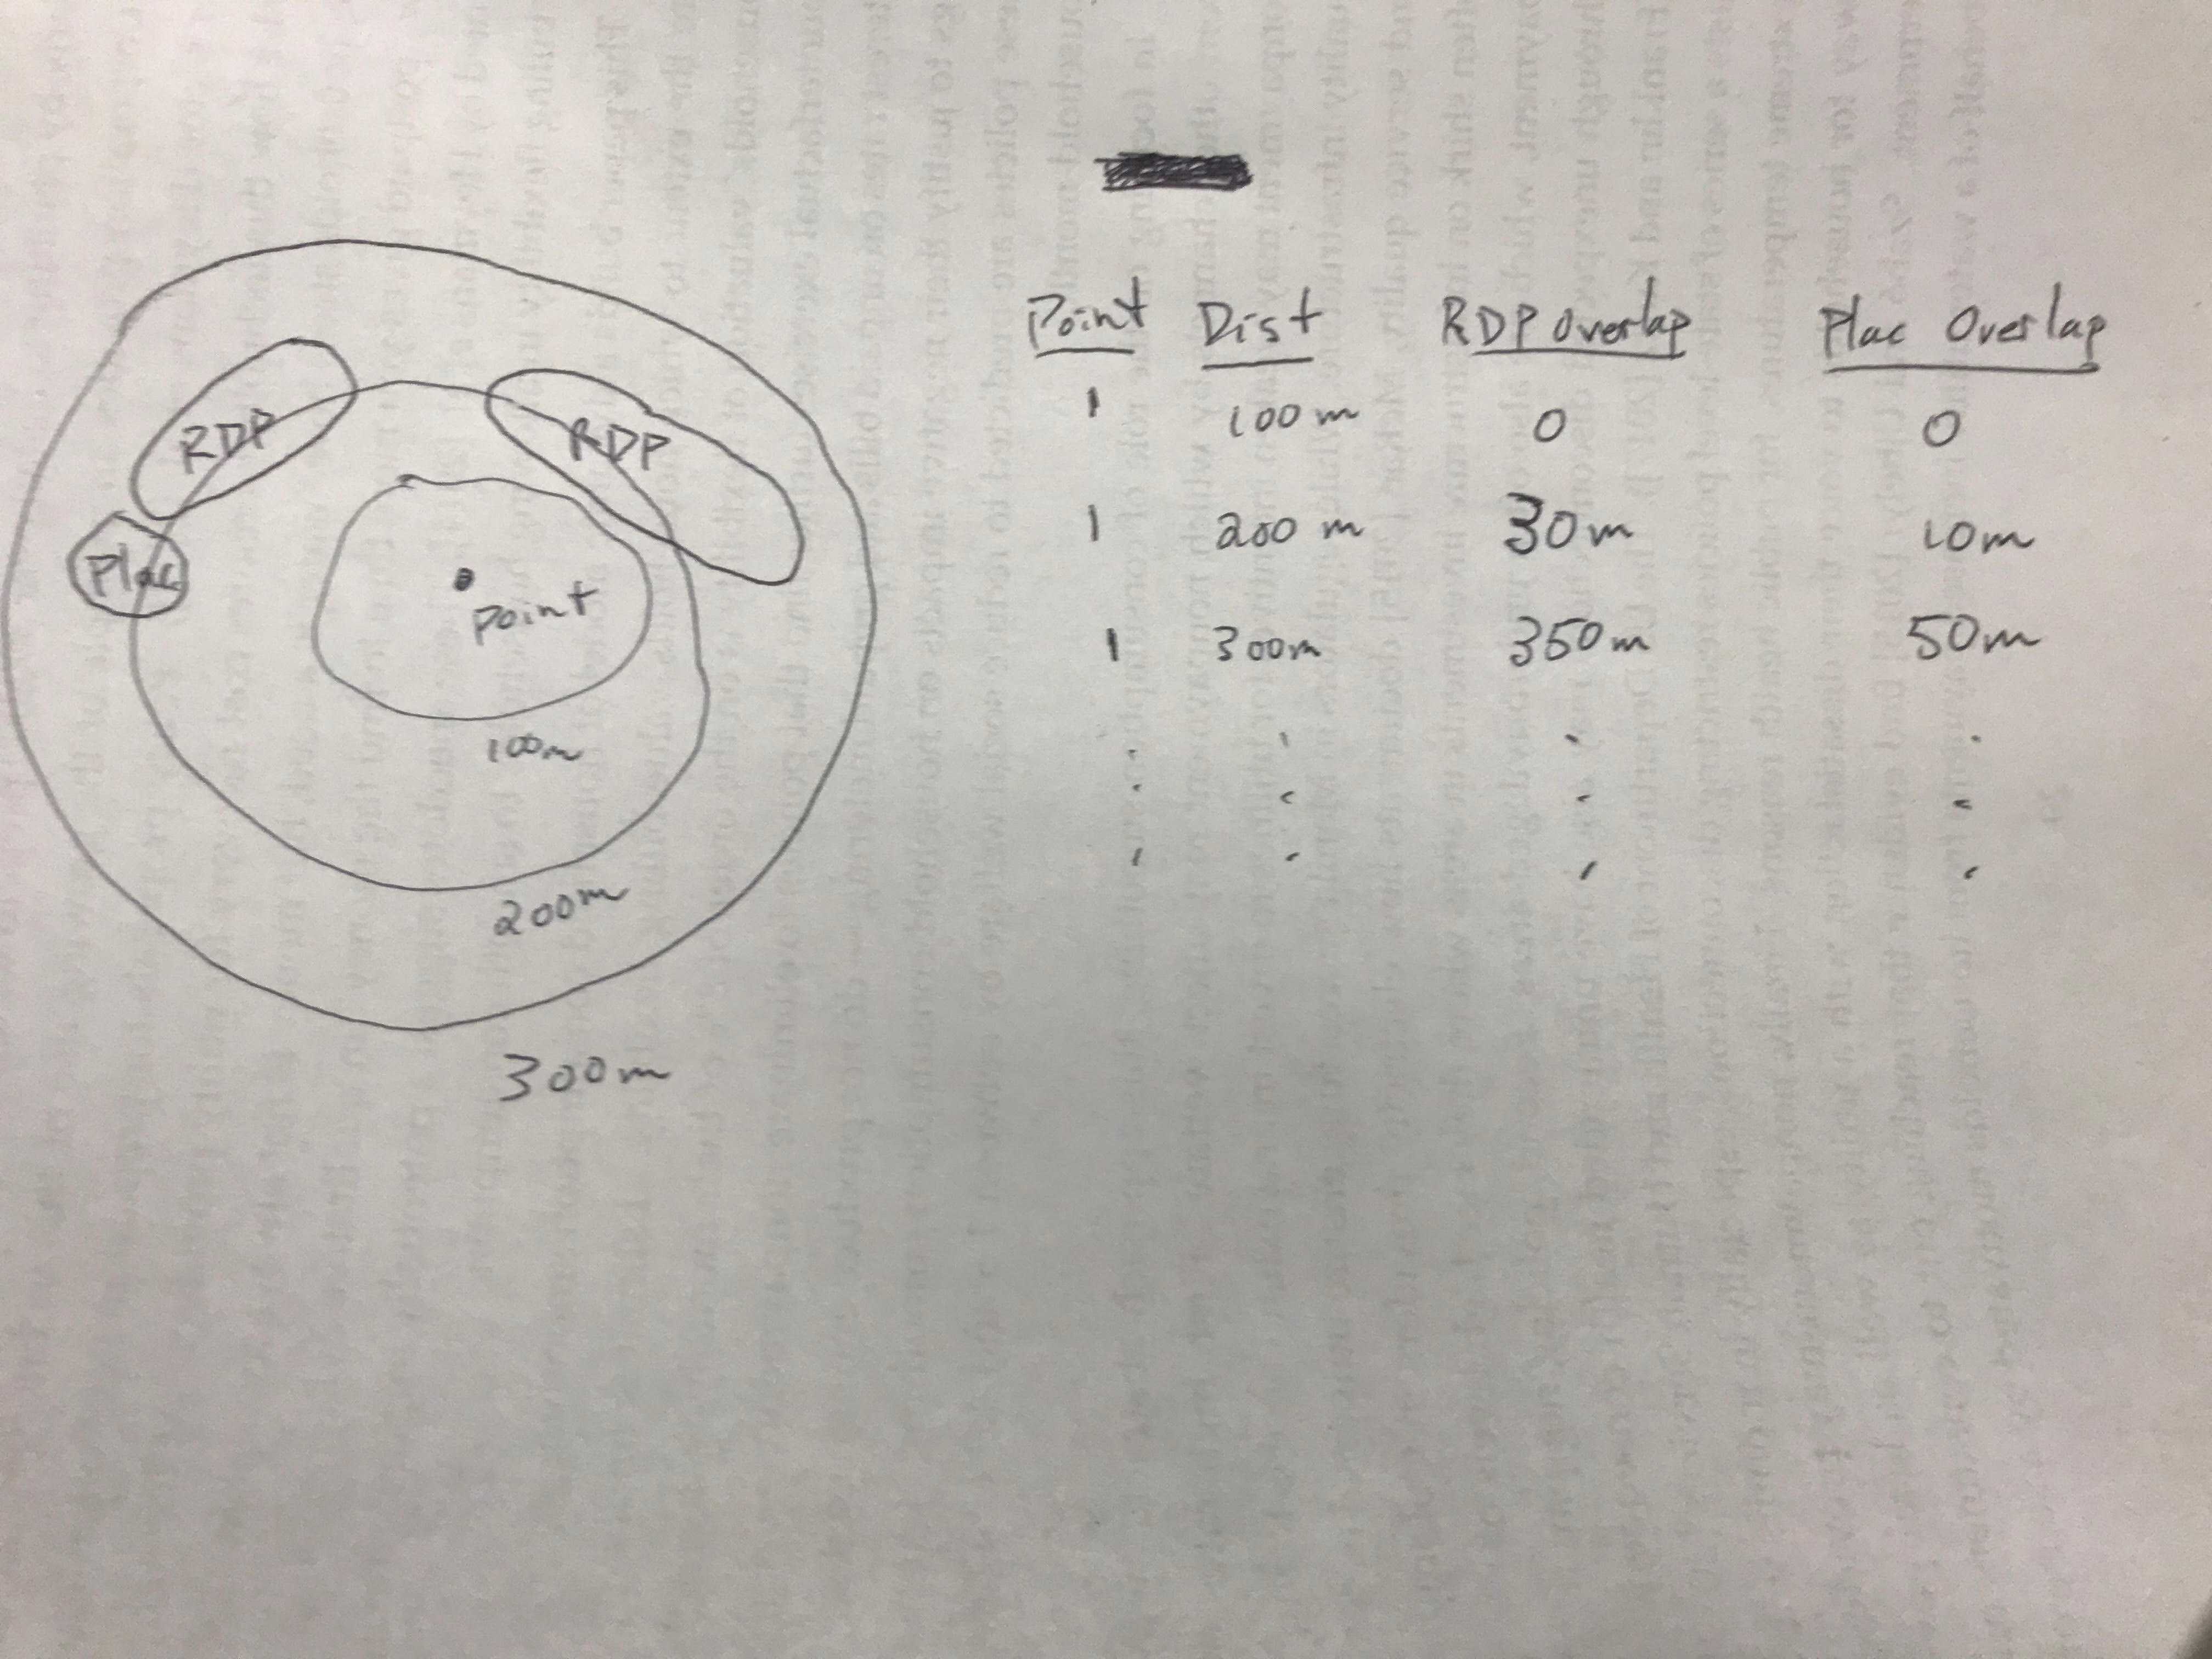
\includegraphics[scale=.11]{figures/overlap_drawing.jpg}
\end{figure}


% reg for post rdp_inside rdp_outside placebo_inside placebo_outside rdp_inside_post rdp_outside_post placebo_inside_post placebo_outside_post if cond2==1, cluster(cluster_reg)

% \pagebreak





% \begin{center}
% \begin{tikzpicture}


% \begin{scope}
%     \clip (1,1) rectangle (0,2);
%     \draw (1,1) circle(3.5cm);
%     %\draw (-1.5,0) -- (1.5,0);
% \end{scope}

% \draw (0,0) -- (2,0) -- (2,2) -- (0,2) -- (0,0);
% \node at (1,1) {RDP};
% \node at (1,1.5) {(1)};
% \node at (-1.5,1) {(4)};
% \node at (-5,1) {(7)};


% %\draw (1,1) circle (3.5cm);
% \draw (1,1) circle (7cm);

% \node at (2,3) {(3)};

% \node at (2,6) {(6)};

% \draw [thick,dash dot] (2,0) -- (4,0) -- (4,2) -- (2,2) -- (2,0);
% \node at (3,1) {Placebo};
% \node at (3,1.5) {(2)};
% \node at (5.5,1) {(5)};
% \node at (9,1) {(8)};

% \draw [thick,dash dot] (3,1) circle (3.5cm);
% \draw [thick,dash dot] (3,1) circle (7cm);

% \end{tikzpicture}
% \end{center}

% \begin{align*}
% Y = \underbrace{post}_{(1)-(8)} + (\underbrace{RDPinside}_{(1)} + \underbrace{RDPoutside}_{(3) + (4)} +   \underbrace{PCBinside}_{(2)} + \underbrace{PCBoutside}_{(3) + (5)})(1+post) + \epsilon
% \end{align*}
% reg for post rdp_inside rdp_outside placebo_inside placebo_outside rdp_inside_post rdp_outside_post placebo_inside_post placebo_outside_post if cond2==1, cluster(cluster_reg)

\end{document}


